\documentclass{beamer}
\usetheme{Madrid}
\usecolortheme{dolphin}
\usefonttheme{structurebold}

\title{Rethinking Refeeding: Cognitive Recovery from Childhood Undernutrition}
\author{Theo Portlock\inst{1} \and Justin O'Sullivan\inst{1}}
\institute{\inst{1}University of Auckland}
\date{03--04--2024}

\begin{document}

\frame{\titlepage}

\begin{frame}{Introduction}
\begin{itemize}
  \item Recovery
\end{itemize}
\end{frame}

\begin{frame}{SAP}
\begin{itemize}
  \item Plot recovery curves
  \item Use Fisher to look for recovery from baseline characteristics
  \item Use RF to look for recovery for each dataset
  \item Use SHAP to look for cross dataset interactions
\end{itemize}
\end{frame}

\begin{frame}{Anthropometric recovery from MAM was achieved in 44\% of children after refeeding}
\begin{center}
  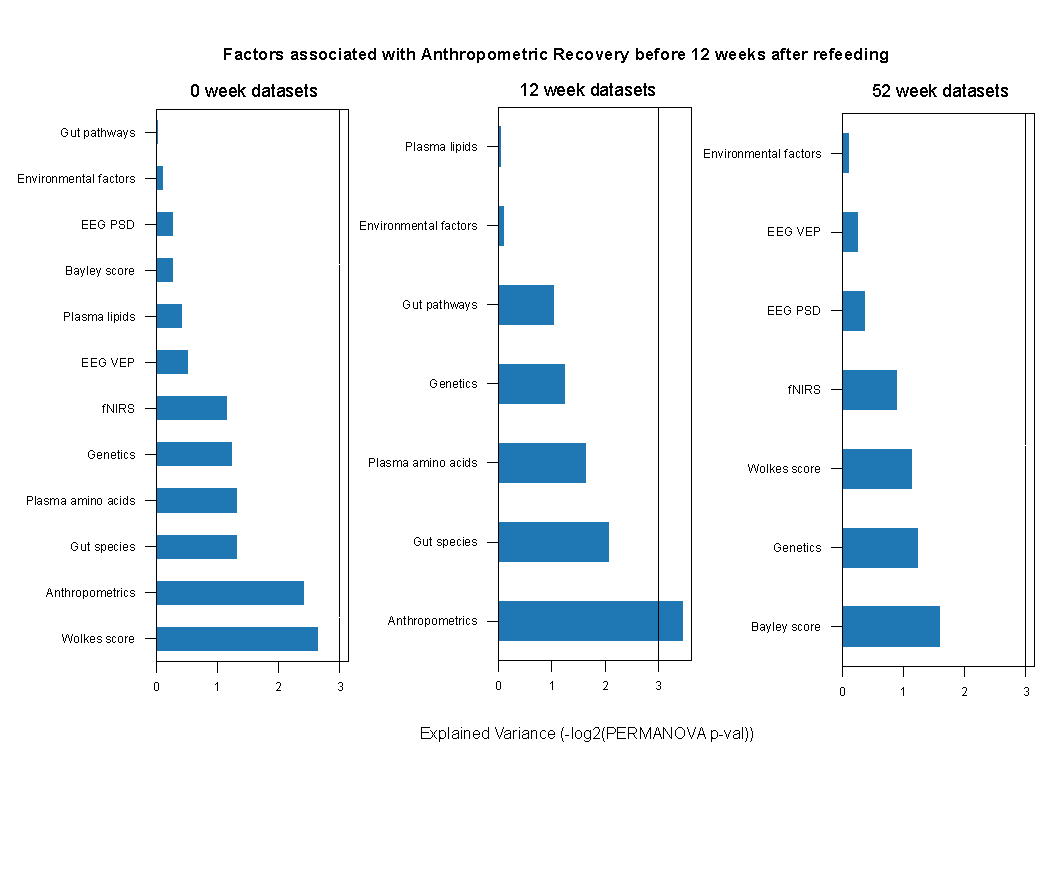
\includegraphics[width=\linewidth]{../../figures/timerecovery.pdf}
\end{center}
\end{frame}

\begin{frame}{Recovery is associated with...}
\begin{center}
  \includegraphics[width=\linewidth]{../../figures/fisher.pdf}
\end{center}
\end{frame}

\begin{frame}{Recovery is difficult to predict}
\begin{itemize}
  \item One-hot encoding
\end{itemize}
\begin{center}
  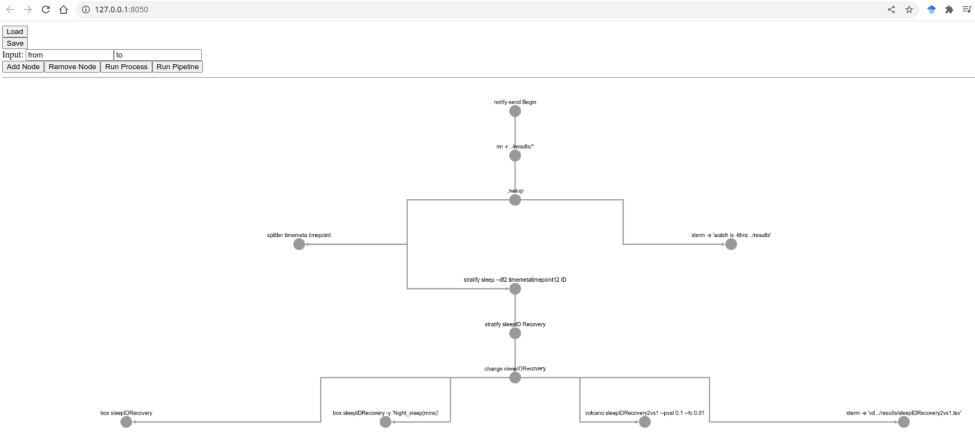
\includegraphics[width=\linewidth]{figures/examplebrowser.pdf}
\end{center}
\end{frame}

\begin{frame}{An interaction predicts recovery}
\begin{center}
  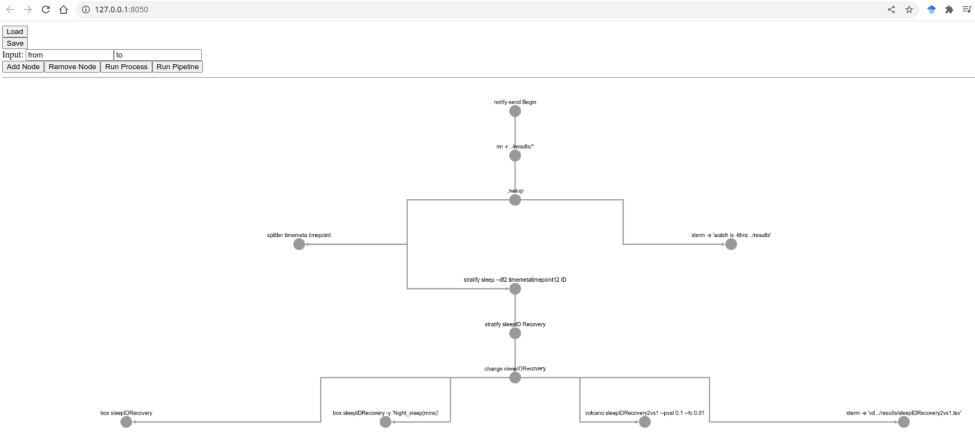
\includegraphics[width=\linewidth]{figures/examplebrowser.pdf}
\end{center}
\end{frame}

\end{document}

